\documentclass{article}
\title{Designate Fracking Wastewater 2AC}
\date{March 6, 2020}
\author{Phineas Greene and LJ Oby}

\usepackage{graphicx}
\usepackage{soul}
\usepackage{url}
\usepackage{booktabs}
\usepackage[colorlinks]{hyperref}
\hypersetup{citecolor=black}
\hypersetup{linkcolor=black}
\hypersetup{urlcolor=blue}
\setuldepth{o}

\addtolength{\oddsidemargin}{-.875in}
\addtolength{\evensidemargin}{-.875in}
\addtolength{\textwidth}{1.75in}

\addtolength{\topmargin}{-.875in}
\addtolength{\textheight}{1.75in}

\begin{document}
\pagenumbering{gobble}
\maketitle
\newpage

\pagenumbering{arabic}
\tableofcontents
\newpage

%<<<<<<<<<<<<<<<<<<<<<<<<<<<<<<<<<<<<<OQ>>>>>>>>>>>>>>>>>>>>>>>>>>>>>>>>
\section{Opening Quotes}

\subsection{California Pits}
\paragraph{}
\small
\textit{
\underline{David Hasemyer, Inside Climate News, Nov 20, 2014}
  (InsideClimate News reporter David Hasemyer is co-author of the "Dilbit Disaster: Inside the Biggest Oil Spill You've Never Heard Of," which won the 2013 Pulitzer Prize for National Reporting, and co-authored the 2016 Pulitzer Prize finalist series "Exxon: The Road Not Taken." Prior to joining ICN, Hasemyer had an award-wining tenure at The San Diego Union-Tribune as an investigative reporter. Hasemyer's newspaper work has been recognized by the Associated Press, the Society for Professional Journalists, the Society of American Business Editors and Writers. He also has been a finalist for the Gerald Loeb Award and the Robert F. Kennedy Award for Social Justice and Human Rights. ) “Hazards of Open Pits for Storing Wastewater From Fracking Is Focus of New Study” Published by Inside Climate News
\url{https://insideclimatenews.org/news/20141120/hazards-open-pits-storing-wastewater-fracking-focus-new-study }}
\normalsize
\paragraph{}
``Unlined open-air wastewater pits brimming with the toxic leftovers of fracking and other types of oil and gas development are threatening California's air and water quality, according to a study by two national environmental organizations.''


\subsection{Visiting A Holding Site}
\paragraph{}
\small
\textit{  
\underline{Andrew Grinberg, Clean Water Action/Clean Water Fund, November 2014}
  (Andrew began working with Clean Water in 2006 and in 2016 joined the national program team in Washington DC. From 2011 through 2015, he managed the California oil and gas program, leading statewide efforts to rein in dirty oil and gas activities including disposal of wastewater into unlined pits, underground injection into drinking water sources and unregulated hydraulic fracturing. Andrew has also managed Clean Water Action field canvass programs in San Francisco, Austin, and DC. Andrew was born and raised in San Francisco, attended Occidental College and currently lives in DC.) “In the pits ” Published by Clean Water Action/Clean Water Fund 
\url{https://assets.documentcloud.org/documents/1362974/ca-oil-and-gas-pit-report.pdf} }
\normalsize
\paragraph{}
``Driving north along Highway 33  nicknamed the ``Petroleum Highway''  the group turned off to the east, down a narrow, unmarked and publicly accessible dirt road. A large tanker truck was visible in the distance. It appeared to be dumping water into the ground. Minutes later, the tour approached a gate with a sign reading ``Danger H2S May Be Present.'' Tour members stepped out of the vehicles and were immediately hit with a noxious odor. Several tied bandanas around their mouths and noses to block the fumes. In less than five minutes, many in the group complained of nausea and headaches. The site consisted of a few dozen long narrow ponds, some with standing liquids of different shades of green, brown and black, some dry and empty. The closest pond contained two thick pipes that were discharging steaming black and green fluids to the pond, while vapors visibly rose off the surface of the ponds. A thick black ring of what appeared to be oil rimmed the bank and a shimmering black layer floated on the surface. Pipes connected the first pond receiving the discharge to other, larger ponds stretching out hundreds of yards into the distance.''

%<<<<<<<<<<<<<<<<<<<<<<<<<<<<<<<<<<<<<INHERENCY>>>>>>>>>>>>>>>>>>>>>>>>>>>>>>>>
\section{Inherency/Facts}

\subsection{Fracking Ponds Used}
\paragraph{}
\small
\textit{
\underline{Well Water Solutions, May 2018}
  (Well Water Solutions and Rentals Inc. was founded on the principals of creating strong business to business relationships. We have brought together an extremely talented team of business leaders with oil industry experience, to develop breakthrough solutions and unmatched business to business growth opportunities. We understand that business networking is a vital key to continued growth and business expansion worldwide and that this is also vital for a successful company.) “6 Ways We Can Make Your Frac Site More Environmentally Friendly” Published by Well Water Solutions  \url{https://wwstanks.com/2018/05/25/6-ways-we-can-make-your-frac-site-more-environmentally-friendly/ }}
\normalsize
\paragraph{}
\ul{``Frac ponds are another common reason why fracking companies have a bad reputation with environmentalists and the general population. Frac ponds are essentially open-air pools where wastewater is stored and allowed to evaporate into the air over time. This has obvious air contamination concerns, but these ponds are also dangerous for wildlife that confuse the dirty wastewater with fresh water to drink.} Our above-ground storage tanks are an excellent alternative to these frac ponds, and they are much more environmentally friendly.”

\subsection{Not Considered Hazerdous Waste}
\paragraph{}
\small
\textit{
\underline{Alexandra Zissu, Natural Resources Defense Council, January 27, 2016}
(Alexandra Zissu is the author of The Conscious Kitchen and coauthor of Planet Home, The Complete Organic Pregnancy, and The Butcher's Guide to Well-Raised Meat. She has written for The New York Times, New York magazine, Health, and Bon Appétit. A native New Yorker, she recently moved to the Hudson Valley with her family to be closer to the farms that feed them. You can find her at alexandrazissu.com.) “How to Tackle Fracking in Your Community” Published by Natural Resources Defense Council  \url{https://www.nrdc.org/stories/how-tackle-fracking-your-community}}
\normalsize
\paragraph{}
``\ul{Fracking enjoys loopholes from a number of our bedrock environmental laws,'' Raichel notes. For example, oil and gas waste is not considered a hazardous waste under the Resource Conservation and Recovery Act.} This can make it difficult for concerned citizens to push the needle on a federal level, but it’s still important to call your elected representatives and urge them to close these loopholes. ``Although sweeping change might be slow in coming, staying vocal keeps the pressure on elected officials and industry,” Raichel says. ``As we’ve seen before, if there is enough of a groundswell, it will make a difference.”

\subsection{Exempt From RCRA}
\paragraph{}
\small
\textit{
\underline{Elizabeth Ridlington and Kim Norman, Environment America Research and Policy Center, 2016}
(Elizabeth Ridlington is associate director and senior policy analyst with Frontier Group. She focuses primarily on global warming and clean vehicles and has written dozens of reports on these and other subjects. Her 2018 report Trouble in the Air found that millions of Americans regularly breathe air polluted by smog and particulate pollution, and was covered in the Washington Post, the Atlantic, and National Public Radio. Her report Moving America Forward assessed the impact of state and national policies to reduce global warming emissions, and she has written numerous reports on the benefits of state adoption of stronger vehicle emission standards. Elizabeth graduated with honors from Harvard with a degree in government. She joined Frontier Group in 2002. She lives in Northern California with her husband and son.) “Fracking by the Numbers” Published by Environment America 
\url{https://environmentamerica.org/sites/environment/files/reports/ Fracking\%20by\%20the\%20Numbers\%20vUS.pdf}}
\normalsize
\paragraph{}
``Waste from oil and gas fracking is exempt from the hazardous waste provisions of the federal Resource Conservation Recovery Act (RCRA), exacerbating the toxic threats posed by fracking wastewater. For other industries, the threats posed by toxic waste have been at least reduced due to the adoption of the RCRA, which provides a national framework for regulating hazardous waste. In other industries, illegal dumping is reduced by cradle-to-grave tracking and criminal penalties. Health-threatening practices such as open waste pits, disposal in ordinary landfills, and road spreading are prohibited.”

\subsection{Lack Of Federal Regulation}
\paragraph{}
\small
\textit{  
\underline{Andrew Grinberg, Clean Water Action/Clean Water Fund, November 2014}
  (Andrew began working with Clean Water in 2006 and in 2016 joined the national program team in Washington DC. From 2011 through 2015, he managed the California oil and gas program, leading statewide efforts to rein in dirty oil and gas activities including disposal of wastewater into unlined pits, underground injection into drinking water sources and unregulated hydraulic fracturing. Andrew has also managed Clean Water Action field canvass programs in San Francisco, Austin, and DC. Andrew was born and raised in San Francisco, attended Occidental College and currently lives in DC.) “In the pits ” Published by Clean Water Action/Clean Water Fund 
\url{https://assets.documentcloud.org/documents/1362974/ca-oil-and-gas-pit-report.pdf} }
\normalsize
\paragraph{}
``The federal government has largely exempted oil and gas wastes from the Resources Conservation and Recovery Act (RCRA), leaving each state to regulate its own oil and gas waste. This exemption also allows oil and gas waste disposal into class II wells, rather than the more tightly regulated class I injection wells that must meet more stringent construction and siting standards. Without direct federal oversight, California regulators are solely responsible for ensuring oil and gas wastes are handled in a manner that does not threaten water or air quality.''

%<<<<<<<<<<<<<<<<<<<<<<<<<<<<<<<<<<<<<SIGNIFICANCE>>>>>>>>>>>>>>>>>>>>>>>>>>>>>>>>
\section{Significance/Facts}

%******************************Wastewater Used************************************
\subsection{\emph{Uses and Misuses Of Wastewater}}

\subsubsection{Wastewater Used For Irrigation}
\paragraph{}
\small
\textit{
\underline{Environmental Working Group, EcoWatch, Oct. 27, 2016}
(The Environmental Working Group’s mission is to empower people to live healthier lives in a healthier environment. With breakthrough research and education, we drive consumer choice and civic action.) “Why Are California Farmers Irrigating Crops With Oil Wastewater?” Published by EcoWatch \url{https://www.ecowatch.com/california-crops-oil-wastewater-2064638069.html}}
\normalsize
\paragraph{}
``In the last three years, farmers in parts of California's Central Valley irrigated nearly 100,000 acres of food crops with billions of gallons of oil field wastewater possibly tainted with toxic chemicals, including chemicals that can cause cancer and reproductive harm, according to an Environmental Working Group (EWG) analysis of state data.”

\subsubsection{What's In The Wastewater}
\paragraph{}
\small
\textit{
\underline{Award-winning journalist Melissa Troutman, Truthout, February 21, 2019}
( Melissa Troutman is an award-winning journalist and filmmaker who joined Earthworks as a research and policy analyst in 2018. In 2011, she co-founded Public Herald, an investigative news outlet that produced the documentary films Triple Divide, Triple Divide [REDACTED] and INVISIBLE HAND.)``What is fracking and why is it controversial?'' Published by Truthout
\url{https://truthout.org/articles/is-drilling-and-fracking-waste-on-your-sidewalk-or-in-your-pool/}}
\normalsize
\subparagraph{}
``\textbf{Salt.} Flowback and produced water are highly salty. This is because salts are added to the fracturing fluid and also released from the geologic formation. Produced water is so famous for salinity that the hydrocarbon industry often refers to it simply as “saltwater” or “brine.” In the Marcellus Shale, flowback water has been measured at 32,300 mg per liter of sodium. For comparison, EPA guidelines call for a maximum of 20 mg/L in drinking water.
\subparagraph{}
\textbf{Industrial chemicals.} Flowback and produced water contain chemicals that have been injected into the well to facilitate drilling. For example, in the Marcellus Shale, flowback water contains high concentrations of sodium, magnesium, iron, barium, strontium, manganese, methanol, chloride, sulfate and other substances.
\subparagraph{}
\textbf{Hydrocarbons.} Produced water can contain hydrocarbons -- including the toxic substances benzene, toluene, ethylbenzene, and xylene – which can be freed during the drilling process.
\subparagraph{}
\textbf{Radioactive materials.}Water returned to the surface during drilling can carry naturally occurring radioactive materials, referred to by the industry as “NORM.” Flowback and produced water from several large U.S. shale formations have been found to contain the radioactive element radium. When produced water is salty and rich in chlorides, radium tends to be present in higher concentrations.
The EPA allows a maximum of 5 picocuries of radium per liter of drinking water. Produced water has been found to contain radium levels as high as 9,000 picocuries per liter (pCi/g)..”

\subsubsection{Wastewater Being Recycled}
\paragraph{}
\small
\textit{
\underline{Award-winning journalist Melissa Troutman, Truthout, February 21, 2019}
( Melissa Troutman is an award-winning journalist and filmmaker who joined Earthworks as a research and policy analyst in 2018. In 2011, she co-founded Public Herald, an investigative news outlet that produced the documentary films Triple Divide, Triple Divide [REDACTED] and INVISIBLE HAND.)``What is fracking and why is it controversial?'' Published by Truthout
\url{https://truthout.org/articles/is-drilling-and-fracking-waste-on-your-sidewalk-or-in-your-pool/}}
\normalsize
\paragraph{}
``Eureka Resources treats toxic wastewater from drilling and fracking from natural gas in Pennsylvania, and the agency that approves this is the Pennsylvania Department of Environmental Protection (PADEP). In June 2014, Eureka Engineer Jerel Bogdan wrote to PADEP to confirm what, exactly, the company had to do in order to sell the salt byproduct from the company’s waste treatment process to consumers.”

\subsubsection{States Need Federal Help}
\paragraph{}
\small
\textit{
\underline{Award-winning journalist Melissa Troutman, Truthout, February 21, 2019}
( Melissa Troutman is an award-winning journalist and filmmaker who joined Earthworks as a research and policy analyst in 2018. In 2011, she co-founded Public Herald, an investigative news outlet that produced the documentary films Triple Divide, Triple Divide [REDACTED] and INVISIBLE HAND.)``What is fracking and why is it controversial?'' Published by Truthout
\url{https://truthout.org/articles/is-drilling-and-fracking-waste-on-your-sidewalk-or-in-your-pool/}}
\normalsize
\paragraph{}
``You may be wondering how a company like Eureka could get away with repackaging byproducts from fracking and selling them without informing the public about what they really are. But the process is perfectly legal in Pennsylvania through a regulatory mechanism called “de-wasting.” De-wasting essentially means rebranding waste as a new product, often without significant treatment to remove health and environmental hazards.”

%******************************Water Toxic************************************
\subsection{\emph{Contents And Health Harms Of Watewater}}

\subsubsection{Risk of Salt Contamination High}
\paragraph{}
\small
\textit{
\underline{Award-winning journalist Melissa Troutman, Truthout, February 21, 2019}
( Melissa Troutman is an award-winning journalist and filmmaker who joined Earthworks as a research and policy analyst in 2018. In 2011, she co-founded Public Herald, an investigative news outlet that produced the documentary films Triple Divide, Triple Divide [REDACTED] and INVISIBLE HAND.)``What is fracking and why is it controversial?'' Published by Truthout
\url{https://truthout.org/articles/is-drilling-and-fracking-waste-on-your-sidewalk-or-in-your-pool/}}
\normalsize
\paragraph{}
``Eureka tests its frack salt quarterly, but there is no testing of the product for radioactivity and other toxins on a more routine basis. This concerns Daniel Bain, a research professor at the University of Pittsburgh’s Department of Geology and Environmental Science who studies radioactivity. Bain told Public Herald that “all it takes is a little glitch in the process, and you can have a dirty salt at some point.”

\subsubsection{Analysis of Chemichals In Wastewater}
\paragraph{}
\small
\textit{
\underline{Infectious Disease specialist Judy Stone, Forbes, Feb 17, 2017}
(I am an Infectious Disease specialist and author of Resilience: One Family's Story of Hope and Triumph over Evil and of Conducting Clinical Research, the essential guide to the topic.) ``Fracking And What New EPA Means For Your Health'' Published by Forbes   
\url{https://www.forbes.com/sites/judystone/2017/02/17/fracking-and-what-new-epa-means-for-your-health/}}
\normalsize

\begin{table}[h!]
  \begin{center}
    \begin{tabular}{p{2.5cm} | p{1.7cm} | p{3cm} | p{3.5cm} | p{4.2cm}} % <-- Alignments: 1st column left, 2nd middle and 3rd right, with vertical lines in between
      \textbf{Chemical} & \textbf{Type of Additive} & \textbf{Why Used}& \textbf{Non-fracking Uses}& \textbf{Health Problems}\\

      \midrule
      Hydrochloric (muriatic acid) & Acid & helps dissolve rock, and make cracks & swimming pool chemical, toilet bowl cleaner & severe burns to skin, GI and respiratory tract\\
      \midrule
      Polyacrylamide & Reduces friction & minimizes friction in the pipes & water treatment, soil conditioner & nervous system damage, a carcinogen\\
      \midrule
      Methanol&Corrosion inhibitor&prevents corrosion and winterizing agent&used as a solvent and in biodiesel&wood alcohol - can cause blindness and death\\
      \midrule
      Ethylene glycol&Scale inhibitor&prevents scale in pipes&anti-freeze&poisonous\\
      \midrule
      Glutaraldehyde&Biocide&kills bacteria that might be corrosive to pipes&disinfecting medical equipment&commonly cause throat and lung irritation, and asthma\\
      \midrule
      Dimethyl-formamide&Corrosion inhibitor&prevents pipe corrosions&plastics&liver damage, high blood pressure\\
      \midrule
      Isopropanol&Surfactant&increases viscosity of the fluid&"rubbing alcohol," glass cleaner&contact irritation, headache, dizziness\\
      \midrule
      Ammonium persulfate&Breaker&delays breakdown of polymer chains&bleaching, plastics mfg.&respiratory distress, burning on contact

    \end{tabular}
  \end{center}
\end{table}

\subsubsection{Open Holding Realeases VOC's}
\paragraph{}
\small
\textit{
\underline{EARTHWORKS, Febuary 28, 2020}
(Earthworks is a nonprofit organization dedicated to protecting communities and the environment from the adverse impacts of mineral and energy development while promoting sustainable solutions. Earthworks stands for clean air, water and land, healthy communities, and corporate accountability. We work for solutions that protect both the Earth’s resources and our communities.) “Hydraulic Fracturing 101” Published by EARTHWORKS 
\url{https://earthworks.org/issues/hydraulic_fracturing_101/}}
\normalsize

\paragraph{}
``The Pittsburgh University Center for Healthy Environments and Communities (CHEC) has been examining how organic compounds in the shale can be mobilized during fracturing and gas extraction processes. According to the CHEC researchers, these organic compounds are brought to the surface in the fracturing flowback or produced water, and often go into open impoundments (frac ponds), where the wastewater, “will off-gas its organic compounds into the air. This becomes an air pollution problem, and the organic compounds are now termed Hazardous Air Pollutants (HAP’s).”.''

\subsubsection{Open Holding Contaminates Air}
\paragraph{}
\small
\textit{
\underline{EARTHWORKS, Febuary 28, 2020}
(Earthworks is a nonprofit organization dedicated to protecting communities and the environment from the adverse impacts of mineral and energy development while promoting sustainable solutions. Earthworks stands for clean air, water and land, healthy communities, and corporate accountability. We work for solutions that protect both the Earth’s resources and our communities.) “Hydraulic Fracturing 101” Published by EARTHWORKS 
\url{https://earthworks.org/issues/hydraulic_fracturing_101/}}
\normalsize

\paragraph{}
``VOCs not only pose a health concern while in the water, the volatile nature of the constituents means that they can also easily enter the air. According to researchers at the  University of Pittsburgh’s Center for Healthy Environments and Communities, organic compounds brought to the surface in the fracturing flowback or produced water often go into open impoundments (frac ponds), where the volatile organic chemicals can off-gas into the air.''

\subsubsection{More On VOC's}
\paragraph{}
\small
\textit{
\underline{EARTHWORKS, Febuary 28, 2020}
(Earthworks is a nonprofit organization dedicated to protecting communities and the environment from the adverse impacts of mineral and energy development while promoting sustainable solutions. Earthworks stands for clean air, water and land, healthy communities, and corporate accountability. We work for solutions that protect both the Earth’s resources and our communities.) “Hydraulic Fracturing 101” Published by EARTHWORKS 
\url{https://earthworks.org/issues/hydraulic_fracturing_101/}}
\normalsize

\paragraph{}
``Other chemicals, such as 1,2-Dichloroethane are volatile organic compounds (VOCs). Volatile organic constituents have been shown to be present in fracturing fluid flowback wastes at levels that exceed drinking water standards. For example, testing of flowback samples from Texas have revealed concentrations of 1,2-Dichloroethane at 1,580 ppb, which is more than 316 times EPA’s Maximum Contaminant Level for 1,2-Dichloroethane in drinking water.''

\subsubsection{Drinking Water Harms}
\paragraph{}
\small
\textit{  
\underline{Andrew Grinberg, Clean Water Action/Clean Water Fund, November 2014}
  (Andrew began working with Clean Water in 2006 and in 2016 joined the national program team in Washington DC. From 2011 through 2015, he managed the California oil and gas program, leading statewide efforts to rein in dirty oil and gas activities including disposal of wastewater into unlined pits, underground injection into drinking water sources and unregulated hydraulic fracturing. Andrew has also managed Clean Water Action field canvass programs in San Francisco, Austin, and DC. Andrew was born and raised in San Francisco, attended Occidental College and currently lives in DC.) “In the pits ” Published by Clean Water Action/Clean Water Fund 
\url{https://assets.documentcloud.org/documents/1362974/ca-oil-and-gas-pit-report.pdf} }
\normalsize
\paragraph{}
``After learning about an unlined pit site, Clean Water Action began to investigate one pair of pits located near McKittrick in Kern County. By reviewing public documents, and using citizens collected air quality samples, the investigation found documentation of a plume of wastewater containing heavy metals such as boron, high salinity, and other constituents of concern, that has migrated towards high quality, useable groundwater resources. The Central Valley Regional Water Quality Control Board (CVRWQCB or Central Valley Board) has required groundwater testing near the site since 2004. The test results — all public documents — indicate that a plume of wastewater, matching the characteristics of the wastewater in the pits, extends close to a mile to the northeast of the pits. It extends towards the Kern River Flood Channel, the California Aqueduct and high-quality groundwater used for significant agricultural activity. The public documents also indicate a complete lack of enforcement of regulations by the Central Valley''

\subsubsection{Air Quality Harms}
\paragraph{}
\small
\textit{  
\underline{Andrew Grinberg, Clean Water Action/Clean Water Fund, November 2014}
  (Andrew began working with Clean Water in 2006 and in 2016 joined the national program team in Washington DC. From 2011 through 2015, he managed the California oil and gas program, leading statewide efforts to rein in dirty oil and gas activities including disposal of wastewater into unlined pits, underground injection into drinking water sources and unregulated hydraulic fracturing. Andrew has also managed Clean Water Action field canvass programs in San Francisco, Austin, and DC. Andrew was born and raised in San Francisco, attended Occidental College and currently lives in DC.) “In the pits ” Published by Clean Water Action/Clean Water Fund 
\url{https://assets.documentcloud.org/documents/1362974/ca-oil-and-gas-pit-report.pdf} }
\normalsize
\paragraph{}
``Air quality sampling (analyzed by an independent lab) at the pits identified health-threatening and climate-changing pollution. Samples showed the presence of 24 volatile organic compounds (VOC’s), and methane, as well as Benzene and 2-Hexanone, above the Long Term Effects Screening Levels.* After receiving a complaint of noxious odors at the pits, the San Joaquin Valley Air Pollution Control District (the District) responded with a claim of “no threat,” based on self-reported sampling by the operator of the pits. The District did not conduct independent air or water sampling.''

\subsubsection{System Not Accountable}
\paragraph{}
\small
\textit{
\underline{Award-winning journalist Melissa Troutman, Truthout, February 21, 2019}
( Melissa Troutman is an award-winning journalist and filmmaker who joined Earthworks as a research and policy analyst in 2018. In 2011, she co-founded Public Herald, an investigative news outlet that produced the documentary films Triple Divide, Triple Divide [REDACTED] and INVISIBLE HAND.)``What is fracking and why is it controversial?'' Published by Truthout
\url{https://truthout.org/articles/is-drilling-and-fracking-waste-on-your-sidewalk-or-in-your-pool/}}
\normalsize
\paragraph{}
``Here are the four standards Eureka must adhere to, according to Bogden’s letter to PADEP (emphasis added):
A full chemical equivalency analysis of Eureka salt products vs. the salt material currently in use by a given industrial user is \em not required\em. Eureka is required to maintain analytical data/records on file that confirm the salt product meets \em only \em those qualitative requirements listed on the MSDS [Material Data Safety Sheet] for the salt material that a potential buyer is currently procuring from other suppliers. Eureka is \em not required \em to use an accredited third-party analytical laboratory for the qualitative comparison noted above; in-house analytical resources may be used for the comparison if Eureka can demonstrate that those resources are able to generate data sufficient for all parameters included in the comparison. Eureka is \em not required \em to submit the qualitative comparison data to the PADEP for review but rather is required to maintain data/analytical results on file, to be provided upon request by the PADEP.”

\subsubsection{Eating Frack Salt}
\paragraph{}
\small
\textit{
\underline{Award-winning journalist Melissa Troutman, Truthout, February 21, 2019}
( Melissa Troutman is an award-winning journalist and filmmaker who joined Earthworks as a research and policy analyst in 2018. In 2011, she co-founded Public Herald, an investigative news outlet that produced the documentary films Triple Divide, Triple Divide [REDACTED] and INVISIBLE HAND.)``What is fracking and why is it controversial?'' Published by Truthout
\url{https://truthout.org/articles/is-drilling-and-fracking-waste-on-your-sidewalk-or-in-your-pool/}}
\normalsize
\paragraph{}
``Cargill purchased 4,700 tons of salt from Eureka between May 2015 and December 2016. One of Cargill’s meat processing plants, Cargill Meat Solutions in Wyalusing, Pennsylvania, is less than 10 miles away from Eureka’s wastewater treatment facility, and “processes about 1,500 head of cattle per day,” according to Cargill’s website. In an email, PADEP wrote that Cargill “advised the Department” that Eureka’s “[c]rystallized sodium chloride” is used by Cargill “to prepare and treat animal hides, resulting from Cargill’s meatpacking operations. Cargill prepares the animal hides using one of Eureka’s salt products for commercial sale.”

\subsubsection{Wastewater Containst 55 Carcinogens}
\paragraph{}
\small
\textit{
\underline{Award-winning journalist Melissa Troutman, Truthout, February 21, 2019}
( Melissa Troutman is an award-winning journalist and filmmaker who joined Earthworks as a research and policy analyst in 2018. In 2011, she co-founded Public Herald, an investigative news outlet that produced the documentary films Triple Divide, Triple Divide [REDACTED] and INVISIBLE HAND.)``What is fracking and why is it controversial?'' Published by Truthout
\url{https://truthout.org/articles/is-drilling-and-fracking-waste-on-your-sidewalk-or-in-your-pool/}}
\normalsize
\paragraph{}
``But instead of listing what Eureka had to do, the letter confirmed what Eureka didn’t have to do — like test its salt for fracking chemicals, even though in 2017, Yale Public Health found that 55 unique chemical compounds used for fracking are “known, probable, or possible human carcinogens.”

\subsubsection{Issues Stem From Disposal, Not Fracking}
\paragraph{}
\small
\textit{
\underline{Robert P. Murphy, Fraser Institute Publisher, Feb. 13, 2020}
Robert Patrick Murphy (born 23 May 1976) is an American economist. Murphy is Research Assistant Professor with the Free Market Institute at Texas Tech University. He has been affiliated with Laffer Associates, the Pacific Research Institute, the Institute for Energy Research (IER), the Independent Institute, the Ludwig von Mises Institute, and the Fraser Institute. 
\url{https://finance.yahoo.com/news/fraser-institute-news-release-fracking-100010876.html}}

\normalsize
\paragraph{}
``Research has found that risks to drinking water quality are relatively modest, with very few incidents of contamination relative to the enormous boom in fracking operations. And again, problems typically stem from wastewater storage and disposal procedures that can be improved.”

%******************************Open Storage************************************
\subsection{\emph{Use And Harms Of Open Storage}}

\subsubsection{Open Storage Typical}
\paragraph{}
\small
\textit{
\underline{EARTHWORKS, Febuary 28, 2020}
(Earthworks is a nonprofit organization dedicated to protecting communities and the environment from the adverse impacts of mineral and energy development while promoting sustainable solutions. Earthworks stands for clean air, water and land, healthy communities, and corporate accountability. We work for solutions that protect both the Earth’s resources and our communities.) “Hydraulic Fracturing 101” Published by EARTHWORKS 
\url{https://earthworks.org/issues/hydraulic_fracturing_101/}}
\normalsize

\paragraph{}
``Some studies have shown that more than 90\% of fracking fluids may remain underground. \ul{Used fracturing fluids that return to the surface are often referred to as flowback, and these wastes are typically stored in open pits or tanks at the well site prior to disposal.''}

\subsubsection{Open Pits Have a Huge Impact}
\paragraph{}
\small
\textit{
\underline{David Hasemyer, Inside Climate News, Nov 20, 2014}
  (InsideClimate News reporter David Hasemyer is co-author of the "Dilbit Disaster: Inside the Biggest Oil Spill You've Never Heard Of," which won the 2013 Pulitzer Prize for National Reporting, and co-authored the 2016 Pulitzer Prize finalist series "Exxon: The Road Not Taken." Prior to joining ICN, Hasemyer had an award-wining tenure at The San Diego Union-Tribune as an investigative reporter. Hasemyer's newspaper work has been recognized by the Associated Press, the Society for Professional Journalists, the Society of American Business Editors and Writers. He also has been a finalist for the Gerald Loeb Award and the Robert F. Kennedy Award for Social Justice and Human Rights. ) “Hazards of Open Pits for Storing Wastewater From Fracking Is Focus of New Study” Published by Inside Climate News
\url{https://insideclimatenews.org/news/20141120/hazards-open-pits-storing-wastewater-fracking-focus-new-study }}
\normalsize
\paragraph{}
``The California study focused on a series of pits in Kern County, around Bakersfield. The report suggests that hundreds of pits throughout the state and especially those in the heavily drilled Central Valley pose environmental and health threats."We think this is potentially the biggest impact of oil and gas development in California," said Andrew Grinberg, oil and gas program manager for Clean Water Action, in issuing the report. California is the fourth-largest oil-producing state in the U.S., according to the report.  In 2013, the industry produced 8 billion gallons of oil in California while generating 130 billion gallons of wastewater, or approximately 15 barrels of wastewater for every barrel of oil, according to the report.''


\begin{figure}[h!] 
  \subsubsection{Map Of Ponds}
  \paragraph{}
  \small
  \textit{
  \underline{Syndicated Maps, Drilling Maps.com, March 20th, 2018}
  (Drilling maps is a health and safety database. Ponds were located with satellite imagery. The map is nowhere near complete.) “Map of Waste Water Fracking Ponds” Published by Drilling maps.com  
  \url{https://blog.drillingmaps.com/2018/03/map-of-waste-water-fracking-ponds.html}}
  \normalsize


  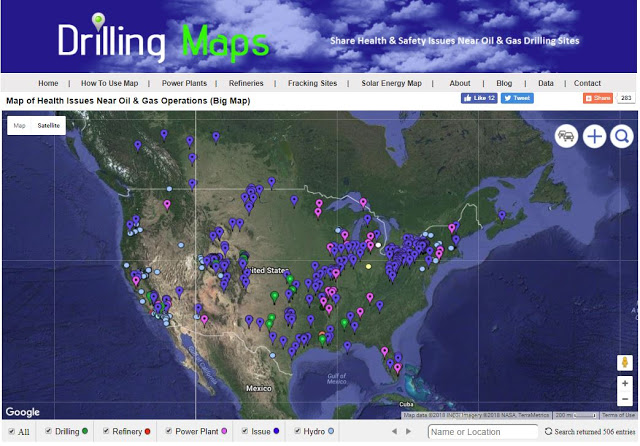
\includegraphics[width=\linewidth]{openholdingmap.jpg}
\end{figure}

\subsubsection{Harms Of Open Holding}
\paragraph{}
\small
\textit{  
\underline{Andrew Grinberg, Clean Water Action/Clean Water Fund, November 2014}
  (Andrew began working with Clean Water in 2006 and in 2016 joined the national program team in Washington DC. From 2011 through 2015, he managed the California oil and gas program, leading statewide efforts to rein in dirty oil and gas activities including disposal of wastewater into unlined pits, underground injection into drinking water sources and unregulated hydraulic fracturing. Andrew has also managed Clean Water Action field canvass programs in San Francisco, Austin, and DC. Andrew was born and raised in San Francisco, attended Occidental College and currently lives in DC.) “In the pits ” Published by Clean Water Action/Clean Water Fund 
\url{https://assets.documentcloud.org/documents/1362974/ca-oil-and-gas-pit-report.pdf} }
\normalsize
\paragraph{}
``In 2013, the industry produced 8 billion gallons of oil in California, and 130 billion gallons of wastewater, or approximately 15 barrels of wastewater for every barrel of oil that is produced. Oil and gas wastewater contains both naturally occurring and added contaminants, including carcinogens, heavy metals, radioactive materials, and salts. In California, oil and gas wastewater is disposed of in four different ways: underground injection into Class II disposal wells; reinjection for enhanced oil recovery (EOR); irrigation of crops; or disposal into unlined pits, also known as sumps. Each presents its own unique challenges and threats to water quality, health, and the environment, but unlined and open-air pits are especially troubling because they are designed to percolate and evaporate toxic chemicals into the environment.''

\subsubsection{Why Open Holding Is Bad}
\paragraph{}
\small
\textit{  
\underline{Andrew Grinberg, Clean Water Action/Clean Water Fund, November 2014}
  (Andrew began working with Clean Water in 2006 and in 2016 joined the national program team in Washington DC. From 2011 through 2015, he managed the California oil and gas program, leading statewide efforts to rein in dirty oil and gas activities including disposal of wastewater into unlined pits, underground injection into drinking water sources and unregulated hydraulic fracturing. Andrew has also managed Clean Water Action field canvass programs in San Francisco, Austin, and DC. Andrew was born and raised in San Francisco, attended Occidental College and currently lives in DC.) “In the pits ” Published by Clean Water Action/Clean Water Fund 
\url{https://assets.documentcloud.org/documents/1362974/ca-oil-and-gas-pit-report.pdf} }
\normalsize
\paragraph{}
``The discharge of wastewater into unlined pits threatens water resources, including potential sources of drinking and irrigation water, and impacts air quality due to the off-gassing of chemicals from the wastewater. The majority of these pits are near waterways, increasing the likelihood that spills and surface-to-groundwater migration will impact water resources. There has been no comprehensive review of locations of pits in relation to high-quality groundwater.''

\subsubsection{Water Should Be Disposed Of Safely}
\paragraph{}
\small
\textit{
\underline{Patrick Hill, TRIPLE POINT, May 23, 2018}
Frac Ponds: Treating Hydraulic Fracturing Wastewater for Reuse” Tripple Point Technologies is a fracking wastewater disposal company. Published by Triple point 
\url{http://www.triplepointwater.com/frac-ponds/\#.Xid7eI7Yo3H}}
\normalsize

\paragraph{}
``Hydraulic fracturing, or fracking, is the process of injecting pressurized water, chemicals, and sand into the ground to extract shale oil and natural gas. While fracking has transformed energy production in the U.S., it requires a lot of water and thus creates a lot of wastewater, which must be treated and disposed of safely. In this video interview, Triplepoint’s resident expert, western regional manager Tom Daugherty, gives the lowdown on fracking wastewater and how frac ponds can be economically upgraded with MARS aeration. Read below for highlights and links to more information.''

%******************************Responses************************************
\subsection{\emph{Responses}}

\subsubsection{Gag Order Regulations}
\paragraph{}
\small
\textit{
\underline{Infectious Disease specialist Judy Stone, Forbes, Feb 17, 2017}
(I am an Infectious Disease specialist and author of Resilience: One Family's Story of Hope and Triumph over Evil and of Conducting Clinical Research, the essential guide to the topic.) ``Fracking And What New EPA Means For Your Health'' Published by Forbes   
\url{https://www.forbes.com/sites/judystone/2017/02/17/fracking-and-what-new-epa-means-for-your-health/}}
\normalsize

\paragraph{}
``But there are many others…and many of these are proprietary and, thanks to the “Halliburton Loophole,” which exempted the injection of these fracking chemicals (now euphemistically called “tools”) from the EPA’s regulation under the Safe Drinking Water Act. In many states, companies don’t even have to disclose what these chemicals are that they are injecting into these wells. Some states, like Pennsylvania, have even had gag orders prohibiting physicians who were given access to these trade secret concoctions in order to take care of their patients from disclosing this information either to other physicians or to the patients themselves!”

\subsubsection{Gag Orders Cause Gaps In Data}
\paragraph{}
\small
\textit{
\underline{Sharon Kelly, DESMOG,  June 25, 2015}
(Sharon Kelly is an attorney and freelance writer based in Philadelphia. She has reported for The New York Times, The Guardian, The Nation, National Wildlife, Earth Island Journal, and a variety of other publications. Prior to beginning freelance writing, she worked as a law clerk for the ACLU of Delaware.) “EPA's New Fracking Study: A Close Look at the Numbers Buried in the Fine Print” Published by DESMOG  
\url{https://www.desmogblog.com/2015/06/25/epa-fracking-study-close-look-numbers-fine-print-details}}
\normalsize

\paragraph{}
``Indeed, the federal government’s recognition that fracking can contaminate drinking water supplies may prove to have opened the floodgates, especially since EPA called attention to major gaps in the official record, due in part to gag orders for landowners who settle contamination claims and in part because there simply hasn’t been enough testing to know how widespread problems have become.”

\subsubsection{Gag Orders Cause Lack Of Numbers}
\paragraph{}
\small
\textit{
\underline{Sharon Kelly, DESMOG,  June 25, 2015}
(Sharon Kelly is an attorney and freelance writer based in Philadelphia. She has reported for The New York Times, The Guardian, The Nation, National Wildlife, Earth Island Journal, and a variety of other publications. Prior to beginning freelance writing, she worked as a law clerk for the ACLU of Delaware.) “EPA's New Fracking Study: A Close Look at the Numbers Buried in the Fine Print” Published by DESMOG  
\url{https://www.desmogblog.com/2015/06/25/epa-fracking-study-close-look-numbers-fine-print-details}}
\normalsize

\paragraph{}
``Once they’ve paid off the victims, the fracking operation is protected and the families are bound to the company, thus, sweeping any evidence of fracking’s dangers under the rug. The practice has proved helpful for the fracking companies in that when giving testimony to Congress, there is no pushback from those who have witnessed and experienced fracking pollution first hand.     “These gag orders are the reason [drillers] can give testimony to Congress and say there are no documented cases of contamination,” said Earthworks organizer Sharon Wilson.  Companies and lawmakers friendly to the companies have even gone so far as to gag doctors from expressing their professional concerns about dangerous fracking chemicals. Last year, a law passed in Pennsylvania that allows doctors to access the listing of the chemicals used in fracking. However, the doctors are prohibited from telling their patients about it.”

\subsubsection{EPA Study Response}
\paragraph{}
\small
\textit{
\underline{Sharon Kelly, DESMOG,  June 25, 2015}
(Sharon Kelly is an attorney and freelance writer based in Philadelphia. She has reported for The New York Times, The Guardian, The Nation, National Wildlife, Earth Island Journal, and a variety of other publications. Prior to beginning freelance writing, she worked as a law clerk for the ACLU of Delaware.) “EPA's New Fracking Study: A Close Look at the Numbers Buried in the Fine Print” Published by DESMOG  
\url{https://www.desmogblog.com/2015/06/25/epa-fracking-study-close-look-numbers-fine-print-details}}
\normalsize

\paragraph{}
``When EPA’s long-awaited draft assessment on fracking and drinking water supplies was released, the oil and gas industry triumphantly focused on a headline-making sentence: “We did not find evidence of widespread, systemic impacts on drinking water resources in the United States.” But for fracking’s backers, a sense of victory may prove to be fleeting. EPA’s draft assessment made one thing clear: fracking has repeatedly contaminated drinking water supplies (a fact that the industry has long aggressively denied).”

\subsubsection{Lobbying Causes Lack Of Change}
\paragraph{}
\small
\textit{
\underline{Janet Redman, Oil change international, October 1, 2017}
(IPS associate fellow Janet Redman is the former director of the Climate Policy Program. For more than a decade, her work has supported the transition from an extractive, fossil-fueled economy to equitable, democratic and local living economies. To that end, Janet uses research, writing and strategic conversations to develop bold ideas in domestic and international policy spaces that redefine what is politically possible. She also practices nurturing deep relationships with grassroots organizations and networks in the global South and North is necessary to align policy advocacy with the goals of social, economics and environmental justice movements. Janet is currently the U.S. Policy Director at Oil Change International and serves on the board of directors of the Global Alliance for Incinerator Alternatives.) “DIRTY ENERGY DOMINANCE: DEPENDENT ON DENIAL” Published by Oil change international
\url{http://priceofoil.org/content/uploads/2017/10/OCI_US-Fossil-Fuel-Subs-2015-16_Final_Oct2017.pdf }}
\normalsize

\paragraph{}
``Repeated proposals by the Obama White House to remove some of the most damaging federal subsidies were thwarted in large part due to the cozy relationship between Congress and the fossil fuel industry. In the 2015-2016 election cycle oil, gas, and coal companies spent \$354 million in campaign contributions and lobbying and received \$29.4 billion in federal subsidies in total over those same years - an 8,200\% return on investment.”

\subsubsection{Fossil Fuels Pay For Status Quo}
\paragraph{}
\small
\textit{
\underline{Janet Redman, Oil change international, October 1, 2017}
(IPS associate fellow Janet Redman is the former director of the Climate Policy Program. For more than a decade, her work has supported the transition from an extractive, fossil-fueled economy to equitable, democratic and local living economies. To that end, Janet uses research, writing and strategic conversations to develop bold ideas in domestic and international policy spaces that redefine what is politically possible. She also practices nurturing deep relationships with grassroots organizations and networks in the global South and North is necessary to align policy advocacy with the goals of social, economics and environmental justice movements. Janet is currently the U.S. Policy Director at Oil Change International and serves on the board of directors of the Global Alliance for Incinerator Alternatives.) “DIRTY ENERGY DOMINANCE: DEPENDENT ON DENIAL” Published by Oil change international
\url{http://priceofoil.org/content/uploads/2017/10/OCI_US-Fossil-Fuel-Subs-2015-16_Final_Oct2017.pdf }}
\normalsize

\paragraph{}
``The fossil fuel industry’s massive spending also paid off in securing \$29.4 billion in total fossil fuel subsidies from the federal government between 2015 and 2016. Put another way, for every \$1 that fossil fuel companies spent on lobbying and campaign finance contributions to Congress, it received more than \$83 back in subsidies – that’s an almost 8,200 percent return on investment to protect the status quo.”

\subsubsection{Trump Administration Involved In Lobbying}
\paragraph{}
\small
\textit{
\underline{Janet Redman, Oil change international, October 1, 2017}
(IPS associate fellow Janet Redman is the former director of the Climate Policy Program. For more than a decade, her work has supported the transition from an extractive, fossil-fueled economy to equitable, democratic and local living economies. To that end, Janet uses research, writing and strategic conversations to develop bold ideas in domestic and international policy spaces that redefine what is politically possible. She also practices nurturing deep relationships with grassroots organizations and networks in the global South and North is necessary to align policy advocacy with the goals of social, economics and environmental justice movements. Janet is currently the U.S. Policy Director at Oil Change International and serves on the board of directors of the Global Alliance for Incinerator Alternatives.) “DIRTY ENERGY DOMINANCE: DEPENDENT ON DENIAL” Published by Oil change international
\url{http://priceofoil.org/content/uploads/2017/10/OCI_US-Fossil-Fuel-Subs-2015-16_Final_Oct2017.pdf }}
\normalsize

\paragraph{}
``To implement this agenda, the Trump Administration has appointed people to key cabinet posts with close ties to the dirty energy industry. Many of these appointees have been pushing for deregulation as lobbyists, lawyers, and industry association experts for years, and are now responsible for the administration’s energy and climate agenda.”

\subsubsection{EPA Involved In Lobbying}
\paragraph{}
\small
\textit{
\underline{Janet Redman, Oil change international, October 1, 2017}
(IPS associate fellow Janet Redman is the former director of the Climate Policy Program. For more than a decade, her work has supported the transition from an extractive, fossil-fueled economy to equitable, democratic and local living economies. To that end, Janet uses research, writing and strategic conversations to develop bold ideas in domestic and international policy spaces that redefine what is politically possible. She also practices nurturing deep relationships with grassroots organizations and networks in the global South and North is necessary to align policy advocacy with the goals of social, economics and environmental justice movements. Janet is currently the U.S. Policy Director at Oil Change International and serves on the board of directors of the Global Alliance for Incinerator Alternatives.) “DIRTY ENERGY DOMINANCE: DEPENDENT ON DENIAL” Published by Oil change international
\url{http://priceofoil.org/content/uploads/2017/10/OCI_US-Fossil-Fuel-Subs-2015-16_Final_Oct2017.pdf }}
\normalsize

\paragraph{}
``Since taking the helm at EPA, Pruitt has met with executives and lobbyists from the oil and gas industry, like the American Petroleum Institute, but largely ignored environmental groups and career EPA staff. He has placed the regulation of the fossil fuel industry squarely in his crosshairs, proposing to review and rescind the Clean Power Plan, delaying rules to curb methane leaks from oil and gas operations, and preparing the legal path to withdrawing the U.S. from the Paris Agreement.”

%******************************Advocasy************************************
\subsection{\emph{Advocacy}}

\subsubsection{Becky Hammer Advocacy}
\paragraph{}
\small
\textit{
\underline{Becky Hammer, NRDC, May 09, 2012}
(Becky Hammer focuses on stormwater runoff, green infrastructure, low-impact development, water-pollution permitting issues, and climate change preparedness. Before joining NRDC in 2009, she interned at the U.S. Environmental Protection Agency. Hammer is a graduate of Harvard College and Harvard Law School. She is based in Washington, D.C.) “Fracking's Aftermath: Wastewater Disposal Methods Threaten Our Health \& Environment” Published by NRDC 
\url{https://www.nrdc.org/experts/becky-hammer/frackings-aftermath-wastewater-disposal-methods-threaten-our-health-environment}}
\normalsize

\paragraph{}
``Some wastewater is stored in open pits (aka “impoundments”). Storage in open pits creates a risk of spills or leakage of wastewater into the ground, potentially contaminating soil, surface water, or groundwater. Additionally, impoundments cause large land disturbances and generate hazardous air pollution as waste evaporates. As a result, impoundments should be banned.”

%<<<<<<<<<<<<<<<<<<<<<<<<<<<<<<<<<<<<<SOLVENCY>>>>>>>>>>>>>>>>>>>>>>>>>>>>>>>>
\section{Solvency}

\subsection{RCRA Overview}
\paragraph{}
\small
\textit{
\underline{National Environmental Trainers, August 12 2019}
(We make individuals and organizations safe, knowledgeable, and more efficient by providing education, training, and workforce management solutions through practical business consulting and advanced technology platforms.) “Resource Conservation and Recovery Act” Published by National Environmental Trainers 
\url{https://www.natlenvtrainers.com/blog/article/resource-conservation-and-recovery-act}}
\normalsize

\paragraph{}
``RCRA's major goals are to reduce waste and provide for the conservation of resources. RCRA's other goals include protecting human health and the environment from potential harm caused by improper waste disposal and (after being amended in 1984) from leaking underground storage tanks. RCRA's management requirements for solid waste and hazardous waste can create a significant administrative and compliance burden on a campus. In most cases, individual states implement and manage the federal RCRA program, as they do with many other federal environmental programs. State environmental protection agencies implement their RCRA programs after receiving approval from the Environmental Protection Agency (EPA). Although these approved state programs operate in lieu of the federal program, EPA retains regulatory oversight over every state program. Although approved programs must provide at least equivalent protection as the federal RCRA standards, states have some flexibility with their own programs. Although no state program can be less restrictive than federal regulations, states may create more stringent requirements by law, rule, or interpretation. RCRA gave EPA and state agencies the authority to require management of hazardous wastes from "Cradle-to-Grave." It also set forth a framework for the management of nonhazardous solid wastes, created a comprehensive underground storage tank (UST) program, and required financial surety for cleanup of releases on operating facilities. In general, the RCRA program established the definitions of solid and hazardous wastes; the design and operational requirements for landfills, incinerators, USTs, etc.; the design, operation, and management requirements for hazardous waste handling and storage containers and structures; a permitting system for entities that create, manage, transport, treat, or dispose of hazardous wastes, including requirements for cleanup of any releases and financial bonding to ensure the availability of funds for possible future cleanups; a cradle-to-grave manifest system used to track hazardous waste; and the liability of the entity (such as a campus) that produces wastes.”

\end{document}